\documentclass[12pt, a4paper]{article}
%\documentclass[runningheads]{llncs}
\usepackage{graphicx}
\usepackage{wrapfig}
\usepackage{subfigure}
\usepackage{multirow}
\usepackage{hyperref}
\usepackage{amsmath}
\usepackage{amssymb}
% \usepackage{ngerman}
\usepackage[ansinew]{inputenc}
\usepackage[left=2.5cm,top=2.5cm]{geometry}
\usepackage[section]{placeins}

\renewcommand\UrlFont{\color{blue}\rmfamily}

\begin{document}

\title{The effect of commen network problems on students academic performance in an elearning-Environment \thanks{Supported by Goethe University Frankfurt a. Main}}

\author{Lucas Laub \inst{1}\orcidID{6621331} \and
Alexander Perekhrest \inst{2}\orcidID{6379748}}

\institute{Goethe University Frankfurt, 60323 Frankfurt a. Main, Germany.}

\maketitle

\begin{abstract}
In the current light of the pandemic the worldwide use
of eLearning-Software experienced an unpresented boom.
We state the question how common network problems influence
the academic performance in an eLearning-Environment.
To provide answers an online questionnaire with deliberate
technical difficulties was constructed. Evaluating the performance
of the test and control group did not show any significant
differences.
\keywords{eLearning  \and Online-Learning \and academic performance.}
\end{abstract}


\section{Introduction}
When trying to transfer an already existing method on a relatively new platform, 
It's important to know the things that come with being on such a platform and the 
possible influences those things might have on the method.\\\\
In day-to-day usage of online platforms and services it's not uncommon to face some 
issues, whether it's execution, connectivity and so on. E-Learning-platforms are not 
particularly different to those. Therefore, we want to discuss, in this paper, to 
which extent these problems can influence the test-results of being on such an 
'issue-infected' platform in contrast to a well running platform with no issues.\\\\
We tried to focus on the most frequent issues we faced in our experience of browsing 
on different platforms, which are defined by HTTP-status-codes, like 400 (Bad Request), 401 
(Unauthorized), 403 (Forbidden), 404 (Not Found), 408 (Request Timeout), as mostly being 
'client-errors', because things like lagging or 100ms more or less ping time are in our 
case of mostly texts and pictures not as important as those client errors.\\\\

\section{Materials and Methods}
\subsection*{Preparations}
The experiment was conducted by creating a software implementing Fig.~\ref{fig1}.
This software allowed the tracking of {\itshape technical problems} introduced by
the software itself as well as the points and answers scored by each participant.
Additionally a room with an adequate number of computers with a fiber-connection
to the server are needed, to rule out uncontrolled network problems.
Half of the computers are manipulated and simulate the network problems with the
use of the software.

\begin{figure}[h]
    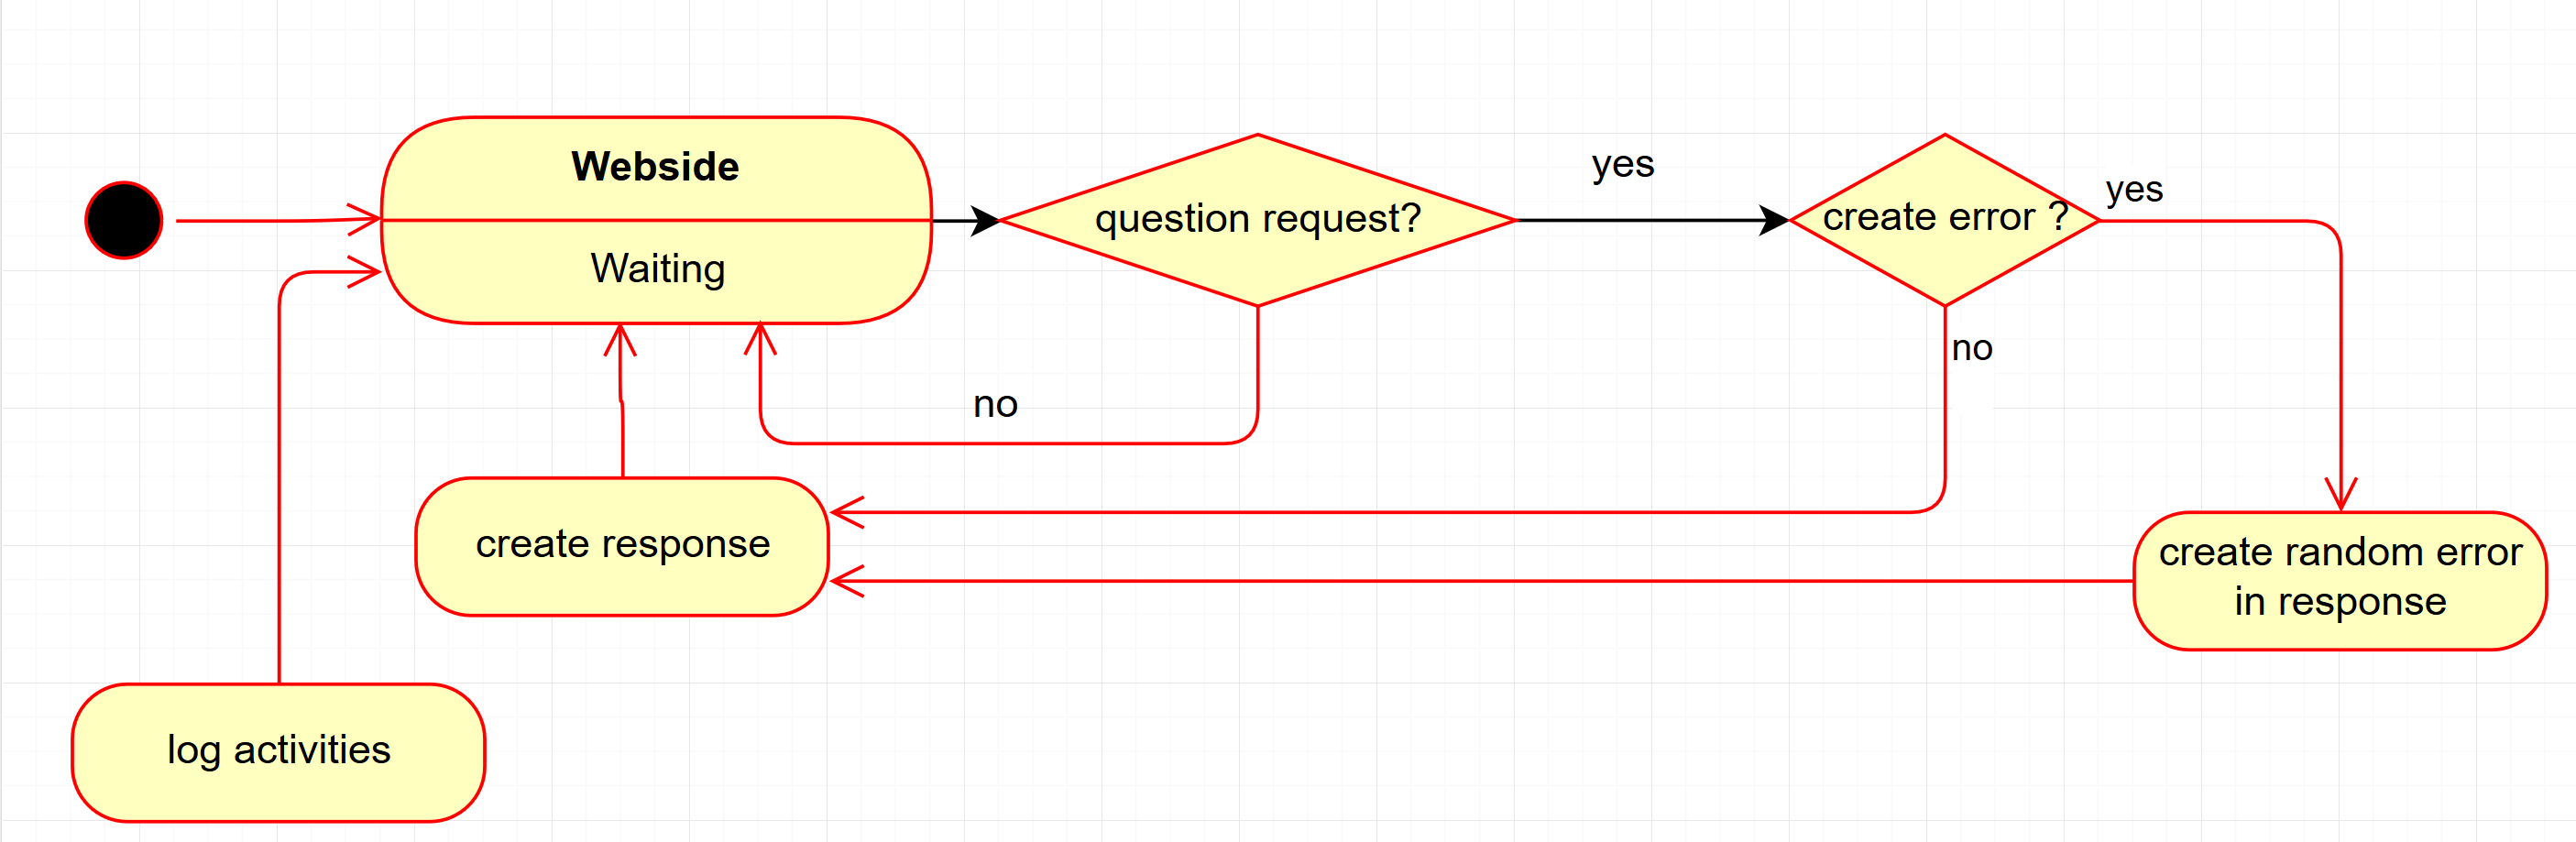
\includegraphics[width=\textwidth]{UML Prototyp.PNG}
    \caption{A logic flow chart , representing how an implementation could operate.
    The black circle is the user interacting with the software. The website would
    consist of two parts. A front-end handling user interaction and the creation of {\itshape bugs}.
    The back-end responsible for saving the collected data and ensuring the front-end
    remains operational.} \label{fig1}
\end{figure}
\newpage
\subsection*{Implementation}
We implemented a possible back-end, which can be used offline. You can find it 
at \url{https://github.com/UebeI2lauf/insertcreativeName/tree/main/code}.
\begin{figure}[h]
    \includegraphics[width=\textwidth]{imp.PNG}
    \caption{The REST API}
\end{figure}
\subsection*{Participants}
The participants are students of the 5th grade and consist of two groups the control group [CG] and
the test group [TG]. Each group is made up by 50 girls and 50 boys for a total of 200 participants.
It should be ensured that both groups prior to the experiment perform academically similar, if not a
comparison post experiment will be difficult.
\newpage
\section{Results}
\begin{figure}[h]
    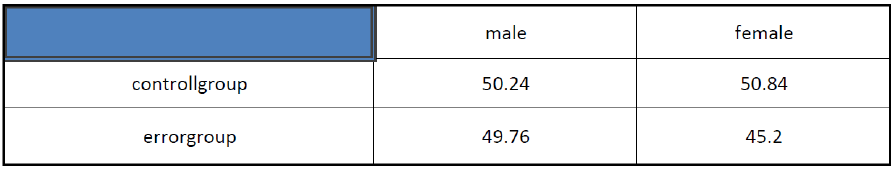
\includegraphics[width=\textwidth]{results.PNG}
\end{figure}
\begin{center}
    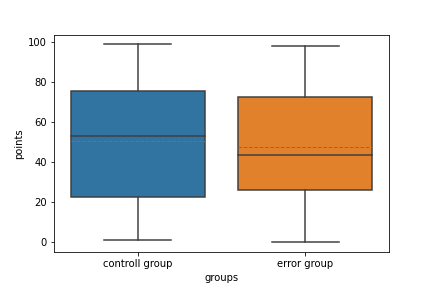
\includegraphics[width=0.5\textwidth]{all.png}
\end{center}
\begin{figure}[h]
    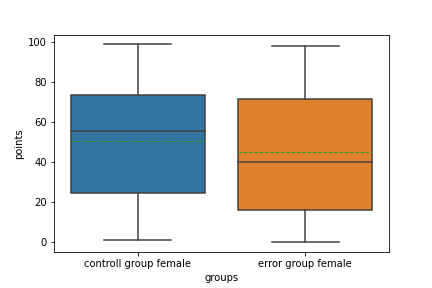
\includegraphics[width=.5\textwidth]{female.png}
    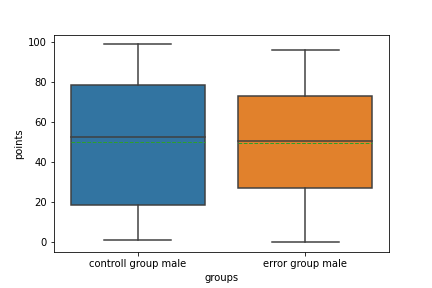
\includegraphics[width=.5\textwidth]{male.png}
    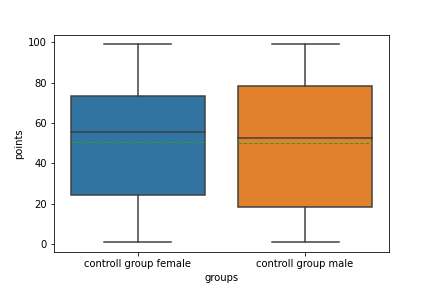
\includegraphics[width=.5\textwidth]{fsav_msav.png}
    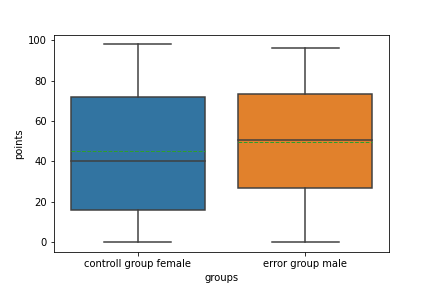
\includegraphics[width=.5\textwidth]{ferr_merr.png}\\\\\\\\
\end{figure}
\begin{figure}[h]
    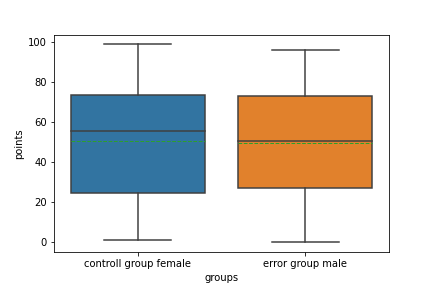
\includegraphics[width=.5\textwidth]{fsav_merr.png}
    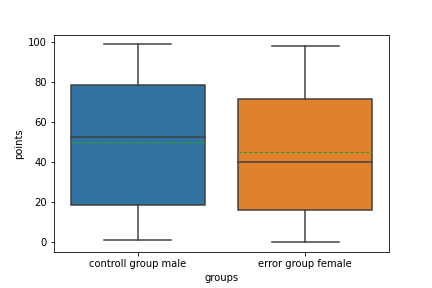
\includegraphics[width=.5\textwidth]{msav_ferr.png}
    \caption{These are the box-plots where we compared the different outcomes with each other. 
    There were 100 reachable points.}
\end{figure}
We also calculated the t- and p-values to see which two groups have the most significant differences. 
We saw the biggest difference between the females from the control group and error group, where we 
got a t-value of 0.949 and a p-value of 0.345. This makes the relationship between error and 
non-error groups not significant enough, because their p-value is larger than 0.05.   

\section{Discussion}
As we can see, the results show not much significance under our circumstances. Even though we 
cannot see a significance, we can see slight worsening of the average scores in the error groups 
than to the control group. But we don't have to forget, that this was a short term test (for 
example 1 hour exam) and we didn't include that many variables like time, age and so on. Having 
such problem-infected websites and platforms can be very frustrating in the long run and may 
make the decline of performance much worse, than we've seen here in our scenario of having 
to enter the 'exam' one time only.  Unfortunately, we couldn't recreate the long-term-scenario 
due to its complexity and sheer number of variables.          
\section{Conclusion}
In this paper we could clearly see the impact of platform-issues on the students performance 
in an exam-scenario and it's not that significant. There might still be certain aspect of long-term-effects,
which we couldn't simulate due to our circumstances, because there was a slight worsening happening when 
comparing our outcomes. It would be very interesting to see, how much significance such things 
like errors will show  in a long run with more variables included. \\\\
Don't neglect setting up your server properly and running it smoothly, so your students will 
thank you for that with better results (in short-term). 

\section{References}
\url{https://github.com/UebeI2lauf/insertcreativeName/tree/main/code}
\end{document}

